\documentclass[12pt]{article}
\usepackage[top=1in,bottom=1in,left=1in,right=1in]{geometry}
\usepackage{alltt}
\usepackage{array}	
\usepackage{graphicx}
\usepackage{tabularx}
\usepackage{verbatim}
\usepackage{setspace}
\usepackage{listings}
\usepackage{amssymb,amsmath, amsthm}
\usepackage{qtree}
\usepackage{hyperref}
\usepackage{oz}
\usepackage[cc]{titlepic}
\usepackage{fancyvrb}
\usepackage{epstopdf}
\usepackage{soul}
\usepackage{array}
\usepackage{graphicx}
\graphicspath{ {./images/} }
\newcolumntype{L}{>{\centering\arraybackslash}m{3cm}}
\usepackage[affil-it]{authblk}

% title
\title{SOEN 331: Introduction to Formal Methods for Software Engineering \\
\textbf{Assignment 2} \\
The Object-Z specification language}

\author{Duc Nguyen - 40064649\\
        Vithura Muthiah - 40062305\\
        Auvigoo Ahmed - 40128901\\
        Ali Hanni - 40157164}
 \affil{Gina Cody School of Computer Science and Software Engineering \\
    Concordia University, Montreal, QC, Canada}
\date{Winter 2021}

\begin{document}
\maketitle

\newpage
\tableofcontents
\newpage


\newpage
\section{Problem 1: State (7 pts)}

\subsection{Description:}

The declaration of the state of the system is defined by

\begin{itemize}
    \item The set of phone numbers (call it \textit{numbers}) that are recorded in contacts
    \item A record of association between names and phone numbers, given by a correspondence
        (call it \textit{recorded}).
\end{itemize}

\begin{enumerate}
    \item Provide a diagram to visualize the state of the system.
    \item Provide a formal definition for numbers.
    \item Does \textit{recorded} have to be captured by a function? What requirements would a function
enforce? Explain in detail.
    \item What is the domain and the codomain of \textit{recorded}?
    \item What type of function should \textit{recorded} be (full or partial)? Explain in detail.
    \item Will \textit{recorded} be an injective, surjective, or bijective? Explain in detail.
    \item Provide a formal definition for \textit{recorded}.
\end{enumerate}

\subsection{Answer:}

\begin{enumerate}
    \item The following figure visualizes the state of the system:
        \begin{figure}[h]
        \centering
        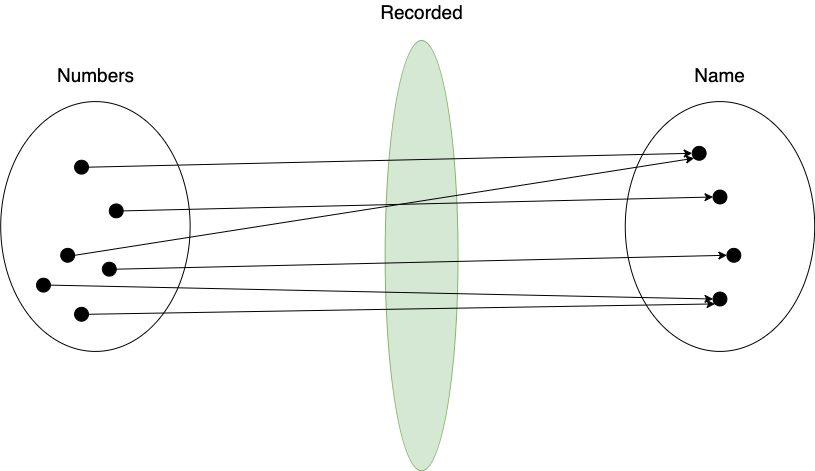
\includegraphics[scale=0.45]{images/Diagram.png}
        \caption{State of the System}
        \label{fig:Diagram}
        \end{figure}
    \item $numbers$ can be formally defined as: \\
    $\{ \forall x, y: numbers | (x \in numbers \wedge y \in numbers) \rightarrow x \neq y \}$
    \item
    \item
    \item As previously stated, the domain of \emph{recorded} is \emph{Numbers}. We know that \emph{Numbers} is the set 
    of all phone numbers recorded in contacts. Since not all elements of \emph{PhoneNumberType} are recorded, we can
    state that \emph{Numbers} is a subset of \emph{PhoneNumberType} as shown in the diagram displayed at \underline{question 1}.
    A partial function \emph{f} is a function that is defined for some subset \emph{A'} of \emph{A}, not forcing mapping for 
    all elements of set A such that $dom f \subset A$. Thus, \emph{recorded} is a partial function.
    \item We know that each element of \emph{Name} (the codomain) has to be associated with at least one element of 
    \emph{Numbers} (the domain). We also know that a name can be associated with multiple phone numbers. This type of 
    function is described as a surjective function. 
    \item The function \emph{recorded} can be formally defined as:\\
    $\{ \forall y \in \emph{Name},   \exists x \in \emph{Numbers} | recorded(x) = y \}$
\end{enumerate}

\newpage
\section{Problem 2: Class Contacts (35 pts)}

\subsection{Description:}
Define a formal specification in Object-Z for class \textit{Contacts} whose interface contains the
following \textit{robust specifications}:

\begin{itemize}
    \item \textbf{MakeNewContact}: Adds a new person to Contacts with a single phone number.
    \item \textbf{AddNumber}: Adds an additional phone number for an existing contact.
    \item \textbf{SearchForNumber}: : Returns a collection of phone numbers for a given person.
    \item \textbf{DeleteNumber}: Deletes an existing number.
\end{itemize}

\subsection{Answer:}

\begin{class}{Contacts}
\also
\upharpoonright (MakeNewContact, AddNumber, SearchForNumber, DeleteNumber) \\
\begin{state}
numbers: \mathbb{P}~PhoneNumberType\\
recorded : NameType \pfun PhoneNumberType\\
\where
numbers = dom~recorded
\end{state} \\
\begin{init}
recorded = \emptyset %\{ \}
\end{init} \\
\begin{op}{MakeNewContactOK}
\Delta (recorded) \\
number?: PhoneNumberType \\
name?: NameType \\
\ST
number? \notin numbers \\
name? \notin ran~recorded \\
recorded' = recorded \cup \{number? \mapsto name? \}
\end{op}\\
\begin{op}{AddNumberOK}
\Delta () \\
\ST
\end{op}\\
\begin{op}{SearchForNumberOK}
\Delta () \\
\ST
\end{op}\\
\begin{op}{DeleteNumberOK}
\Delta () \\
\ST
\end{op}\\
\begin{op}{Success}
response!: Message \\
\ST
response! = 'ok'
\end{op}\\
\begin{op}{NumberExists}
number?: PhoneNumberType \\
response!: Message \\
\ST
number? \in numbers \\
response! = 'Number~already~exists'
\end{op}\
\zbreak
\begin{op}{NameExists}
name?: NameType \\
response!: Message \\
\ST
name? \in ran~recorded \\
response! = 'Name~already~taken'
\end{op}\
\also
MakeNewContact \sdef (MakeNewContactOK \wedge Success) \oplus (NumberExists \lor NameExists) \\
AddNumber \sdef \\
SearchForNumber \sdef \\
DeleteNumber \sdef
\end{class}
\newpage
\section{Problem 3: Class Contacts2 (8 pts)}

\subsection{Description:}
Subclassify \textbf{Contacts} to introduce class \textbf{Contacts2} that behaves exactly like \textbf{Contacts},
while introducing a robust operation to search for a person, given a phone number through
operation \textbf{SearchForPerson}.

\subsection{Answer:}



\end{document}
